\section{Flexibility Trap}
\label{sec:rethink_value_of_AO}
이 절에서는 arbitrary-order generation의 유연성이 더 높은 reasoning 잠재력으로 이어지는지 실증적으로 검증한다.
우리는 두 가지 decoding 모드를 비교한다: 낮은 confidence의 remasking을 사용하는 표준 diffusion decoding을 따르는 \emph{Arbitrary Order}~\cite{nie2025large,zhao2025d1,fastdllm}와 arbitrary-order 유연성을 비활성화하고 생성을 엄격히 left-to-right decoding으로 제한하는 \emph{AR Order}이다. 
우리는 기존 diffusion LLM 연구에서 일반적으로 사용되는 실험 설정을 채택한다: 최대 256 tokens를 256 steps에 걸쳐 decoding하고, semi-autoregressive block size는 32로 둔다.
Sampling temperature는~\cite{yue2025does}와 같이 0.6으로 설정한다. Prompt template은~\cite{zhao2025d1}를 따른다.
대안적인 temperature와 sampling 구성에서의 결과는 Appendix~\ref{app:boundary_ablations}로 미룬다.

\subsection{Arbitrary Order는 Reasoning 잠재력을 제한할 수 있다}
\paragraph{Pass@$k$ analysis.}
먼저 네 가지 reasoning benchmarks인 GSM8K, MATH-500, HumanEval, MBPP에서 세 가지 대표적인 dLLMs: LLaDA-Instruct~\cite{nie2025large}, Dream-Instruct~\cite{ye2025dream}, LLaDA 1.5~\cite{zhu2025llada}에 대해 Pass@$k$ metric을 사용해 reasoning 잠재력을 평가한다.
Figure~\ref{fig:passk_comparison}에 보이듯, arbitrary order는 $k=1$에서 종종 경쟁력 있고 많은 경우 더 나은 성능을 달성하지만, AR mode와 비교하면 scaling curve가 눈에 띄게 더 평평하다. $k$가 증가함에 따라 AR mode는 더 많은 정답 solution을 찾아내는 더 강한 능력을 보인다. 



\begin{figure}[t]\centering
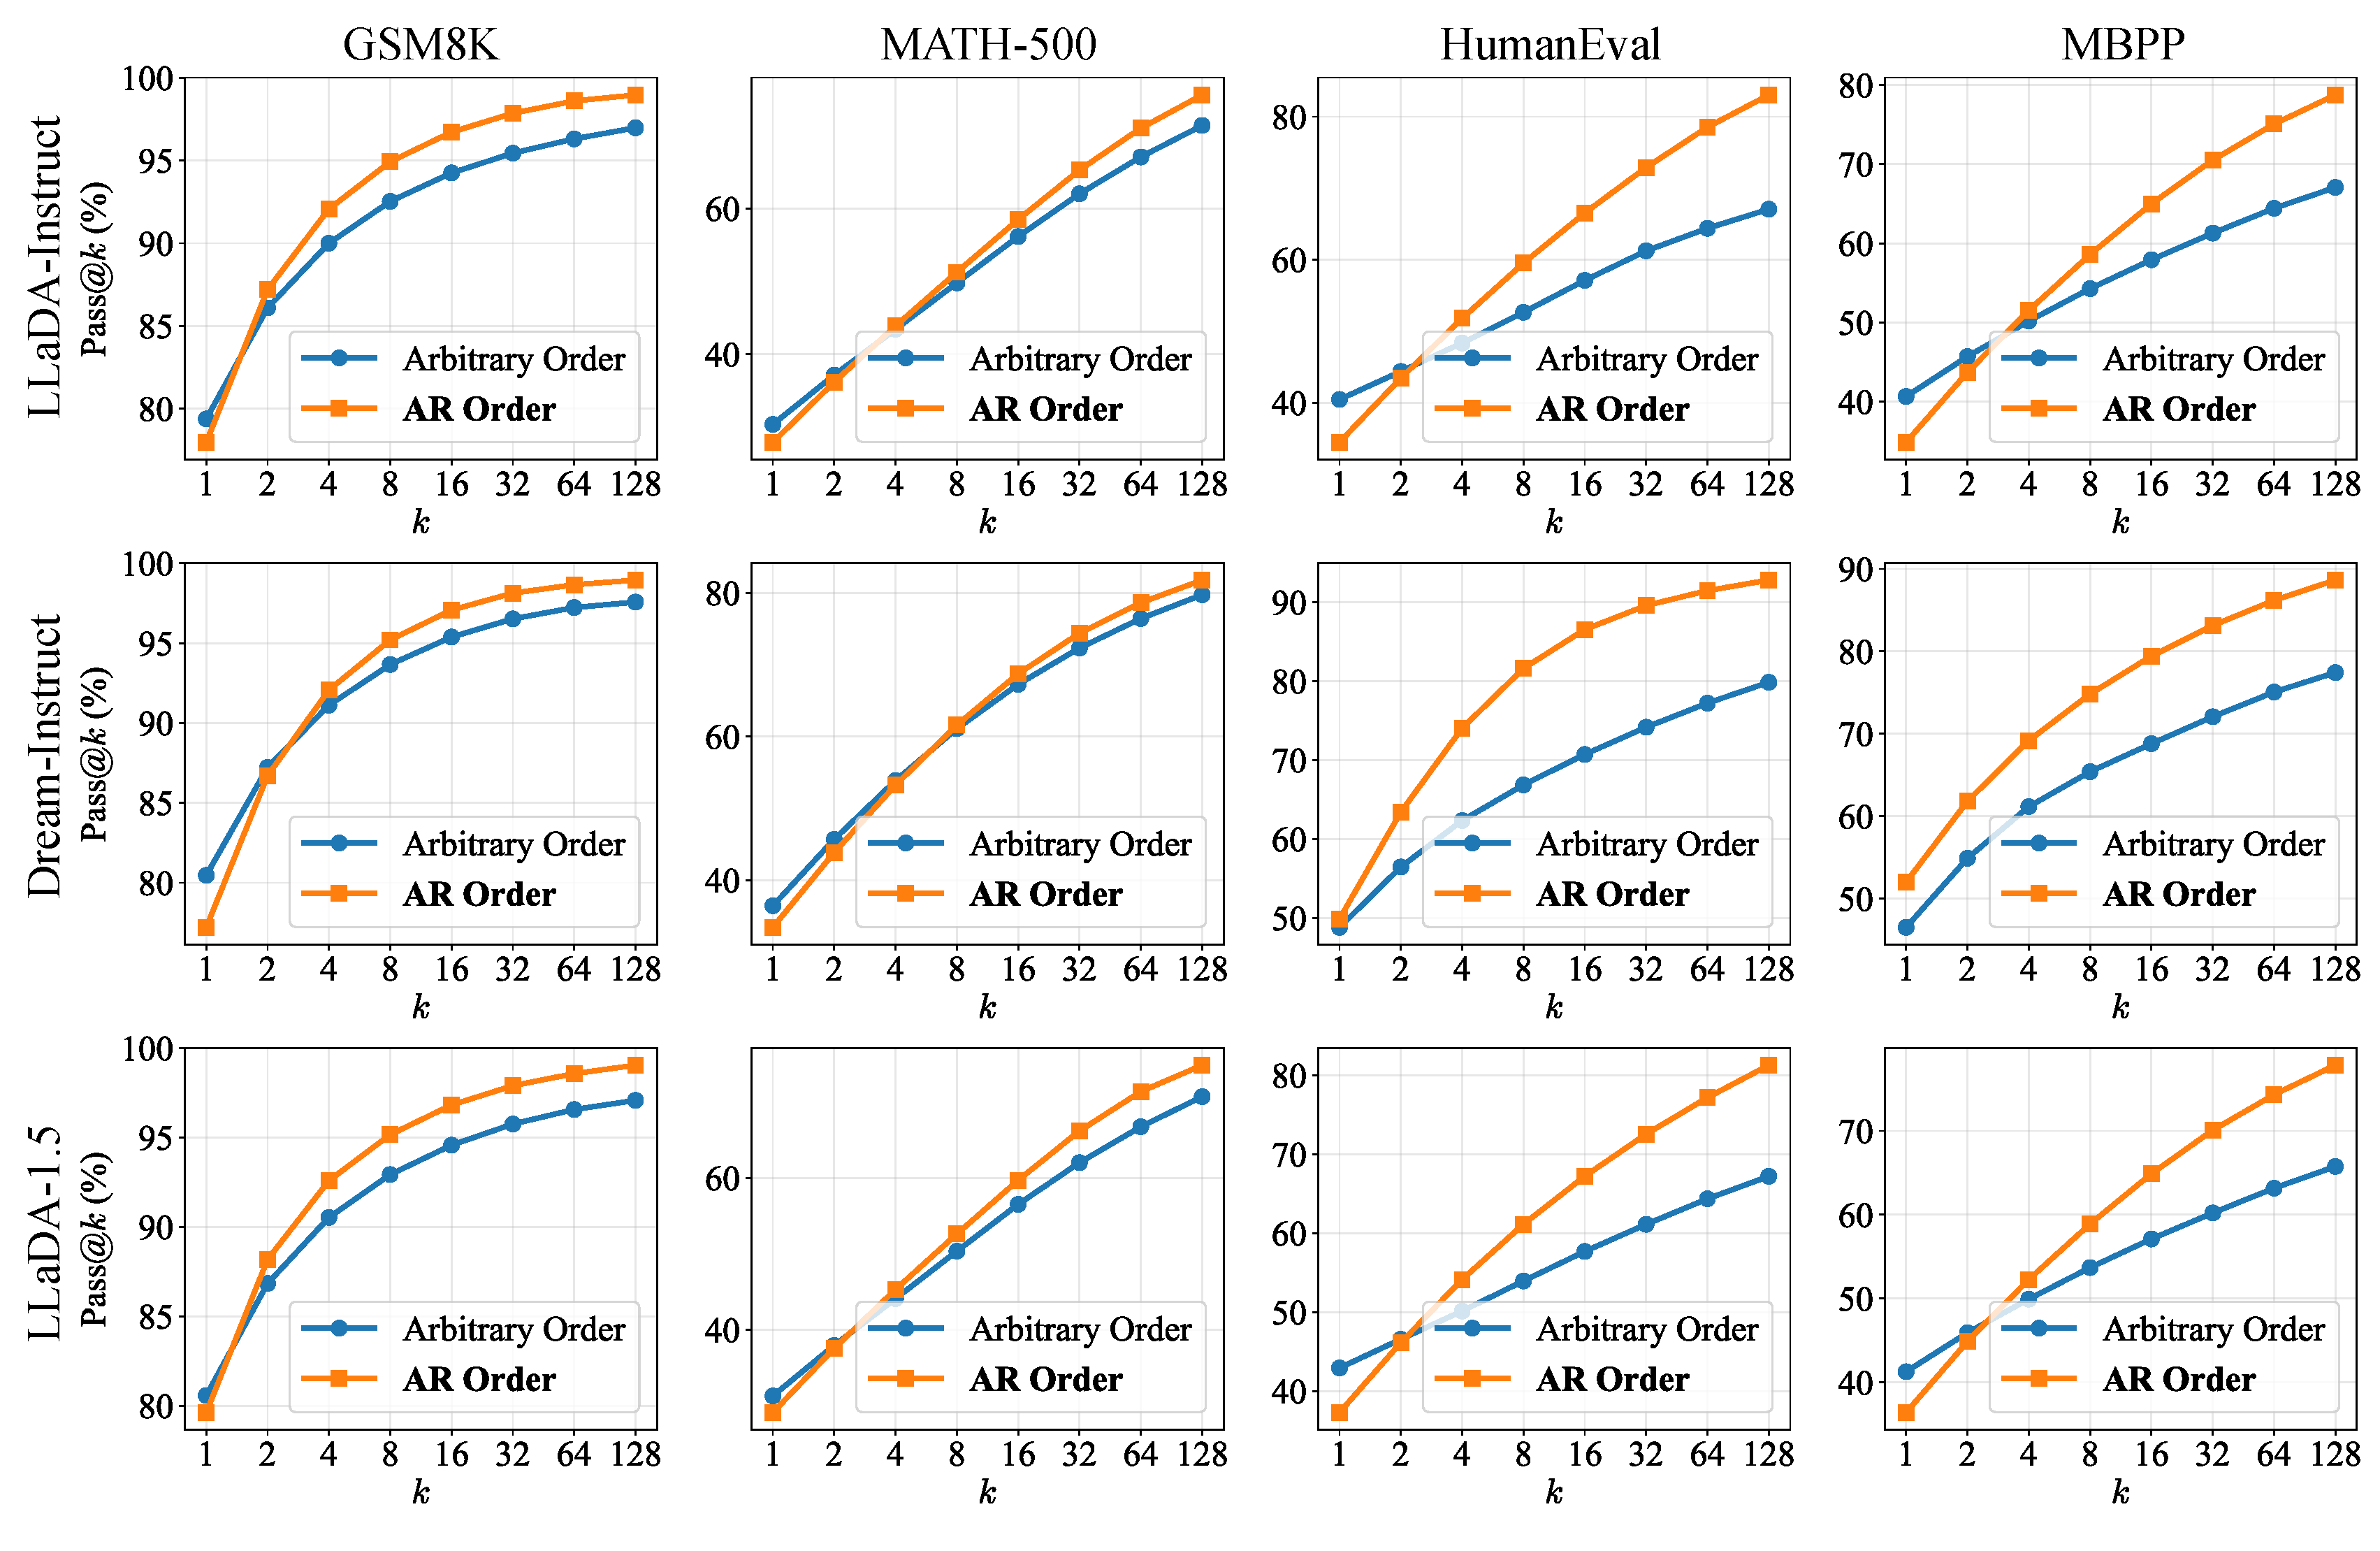
\includegraphics[width=\linewidth]{figures/passk_comparison.pdf}
\vskip -.15in
\caption{
    \textbf{Pass@$k$로 측정한 reasoning 잠재력.} arbitrary order는 single-shot 설정($k=1$)에서 경쟁력이 있지만, AR Order에 비해 더 평평한 scaling curves를 보인다.
    이러한 관찰은 서로 다른 dLLMs와 일반 reasoning benchmarks 전반에서 일관된다.
    \label{fig:passk_comparison}
}
\end{figure}

\begin{wrapfigure}{r}{0.52\textwidth}
    \centering
    \vskip -0.22in
    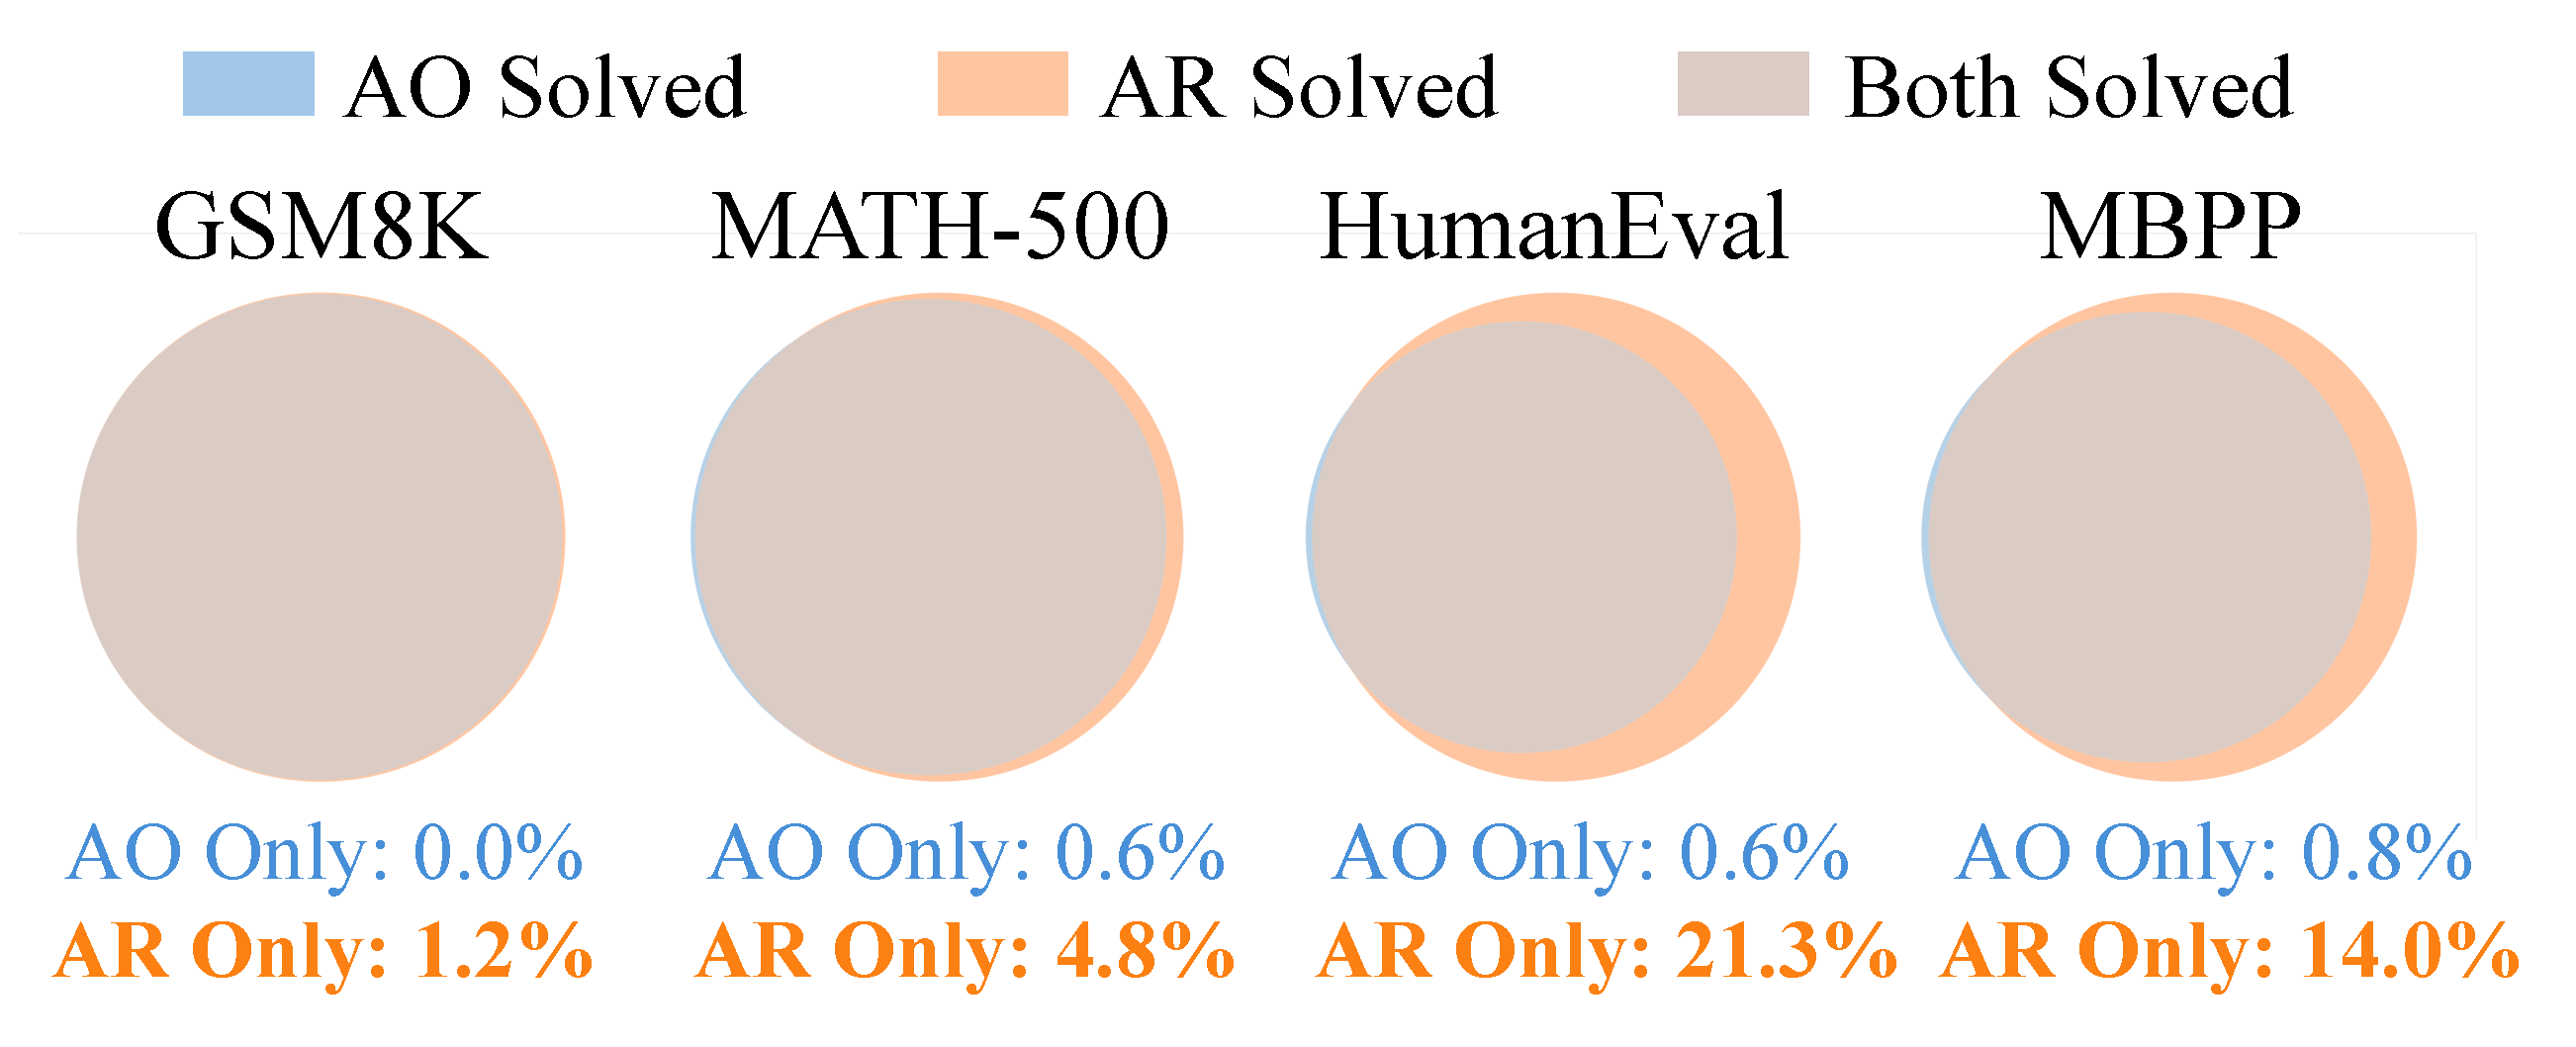
\includegraphics[width=\linewidth]{figures/venn.pdf}
    \vskip -.1in
    \caption{
        \textbf{Pass@$1024$로 측정한 solution space coverage.} arbitrary order (AO)로 풀 수 있는 문제들은 대체로 AR Order가 해결한 문제들의 subset이다.
        결과는 LLaDA-Instruct로 측정했다.
    }
    \label{fig:ar_vs_diff_venn}
    \vskip -0.18in
\end{wrapfigure}


\paragraph{Solution space coverage.}
arbitrary order가 효율은 낮더라도 다른 solution space를 탐색하며, 이것이 낮은 reasoning 잠재력을 설명할 수 있지 않을까 생각할 수 있다.
우리는 LLaDA-Instruct를 사용해 $k=1024$에서 solution coverage를 분석하여 이를 검증한다. 
Figure~\ref{fig:ar_vs_diff_venn}에 보이듯, arbitrary-order generation을 통해 얻은 solutions는 AR decoding이 발견한 solutions와 대체로 겹치며, 실제로는 더 작은 subset을 이룬다는 것을 발견했다.
예를 들어 HumanEval에서 문제의 21.3\%는 AR에 의해서만 해결되는 반면, 그 반대 경우는 드물다(0.6\%).
arbitrary-order generation은 이론적으로 더 큰 solution space를 함의하지만, 실제 sampling regime에서 효과적으로 도달 가능한 solution들의 집합은 더 제약적인 것으로 보인다.


\begin{wrapfigure}{r}{0.46\textwidth}
    \centering
    \vskip -0.28in
    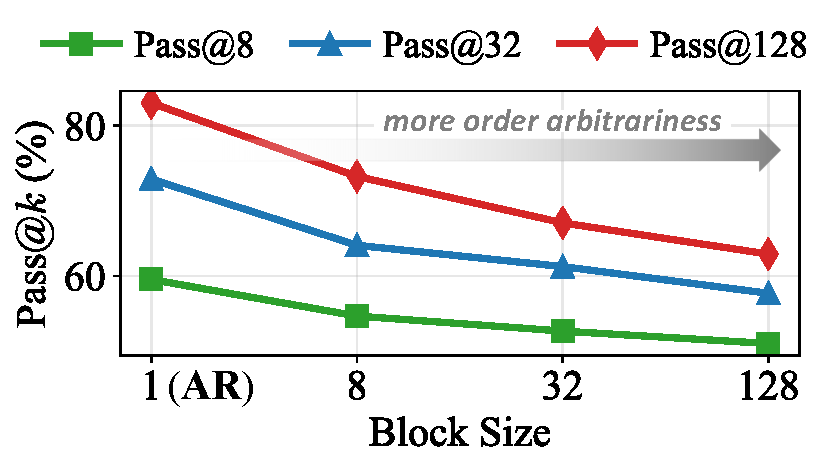
\includegraphics[width=\linewidth]{figures/block_size_humaneval.pdf}
    \vskip -0.15in
    \caption{
        \textbf{더 큰 arbitrariness, 더 낮은 potential.}
        우리는 서로 다른 수준의 order arbitrariness에 대해 semi-autoregressive decoding block size $B$를 sweep한다: $B=1$은 순수 AR order를 복원하고, 더 큰 $B$는 sampler가 다음에 어떤 position을 resolve할지 선택하는 데 더 많은 자유를 부여한다. 결과는 LLaDA-Instruct로 HumanEval에서 측정했다.
        \label{fig:arbitrary_block_size_analysis}
    }
    \vskip -0.4in
\end{wrapfigure}
\paragraph{더 큰 arbitrariness, 더 낮은 potential.}
지금까지 우리는 arbitrary order와 AR order를 두 극단으로 대비했지만, arbitrariness의 정도는 이분법적이지 않다. dLLMs~\cite{nie2025large,ye2025dream}의 semi-autoregressive protocol은 block size $B$를 통해 이를 제어한다: sequence는 크기 $B$의 blocks로 나뉘고, 각 block 안에서 model은 unmask할 tokens를 adaptive하게 선택한다.
따라서 $B$는 model이 다음 position을 자유롭게 선택할 수 있는 범위를 정하며, $B=1$은 자유도를 남기지 않고(순수 AR order) 더 큰 $B$는 더 arbitrary한 decoding을 허용한다; 위의 실험에서는~\cite{zhao2025d1}를 따라 $B=32$를 사용했다.
이제 $B$를 sweep하여 arbitrariness의 정도가 reasoning 잠재력에 어떤 영향을 미치는지 조사한다.

Figure~\ref{fig:arbitrary_block_size_analysis}에 보이듯, 추세는 일관되고 단조롭다: 모든 $k \in \{8, 32, 128\}$에 걸쳐 $B$가 커질수록 Pass@$k$는 감소한다. 이는 그 효과가 두 극단적 설정에 묶인 것이 아니라 일관적임을 시사한다: 이 설정에서는 더 낮은 arbitrariness가 더 높은 reasoning 잠재력과 일관되게 연관된다.

\subsection{Mechanism: Entropy Degradation}


\begin{wrapfigure}{r}{0.30\textwidth}
    \centering
    \vskip -0.15in
    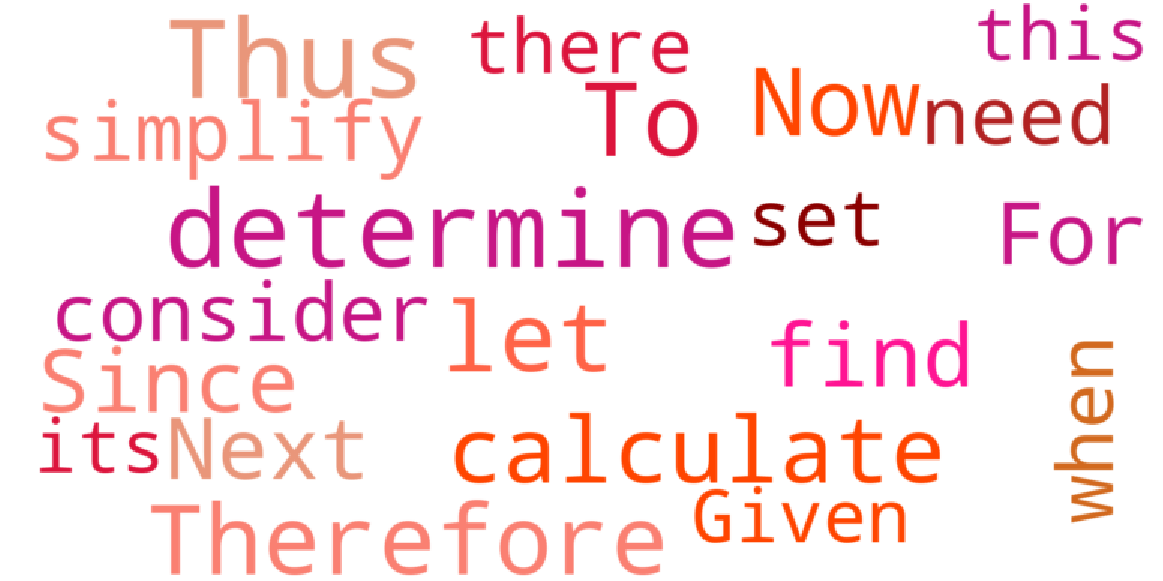
\includegraphics[width=\linewidth]{figures/bypass_words.pdf}
    \vskip -0.10in
    \caption{
        arbitrary order에서 \textbf{자주 bypass되는 tokens}는 보통 논리적 연결어와 전환어이다.
        결과는 LLaDA-Instruct로 MATH-500에서 측정했다.
        \label{fig:bypass_words}
    }
    \vskip -0.14in
\end{wrapfigure}
\paragraph{Adaptive decoding은 logical forks를 bypass한다.}
dLLMs의 이론적으로 더 큰 solution space가 실제로는 왜 collapse되는지 이해하기 위해, 두 decoding 모드가 어떻게 작동하는지 더 자세히 살펴본다.
AR order에서 model은 각 step마다 가장 왼쪽의 unknown token을 엄격히 resolve하도록 제약되어, uncertainty가 발생하는 순간 이를 직면하게 된다.
반대로 arbitrary order는 model confidence를 바탕으로 update할 tokens를 \emph{adaptive하게} 선택하며, ``어려운'' ones를 bypass하는 동안 높은 certainty를 가진 ``쉬운'' tokens를 우선적으로 생성한다.
자주 bypass되는 tokens를 살펴보면 명확한 pattern이 드러난다:
Figure~\ref{fig:bypass_words}에 보이듯, diffusion sampler는 ``Therefore'', ``Thus'', ``Since''와 같은 논리적 접속어와 전환 표지를 불균형적으로 뒤로 미룬다.
기존 연구는 그러한 tokens가 종종 높은 entropy를 가지며(dLLMs에서도 마찬가지이다; Figure~\ref{fig:bypass_compare} 참조), 이후 reasoning 방향을 결정하는 분기점으로 기능하는 ``reasoning sparks'' 또는 ``logical forks''로 작용한다는 것을 보였다~\cite{wang2025beyond,cheng2025reasoning,huang2025low}.
기존 language models에서는 이러한 tokens를 high-entropy state로 유지하는 것이 reasoning space의 효과적인 exploration에 중요하다~\cite{wang2025beyond}.

\begin{wrapfigure}{r}{0.5\linewidth}
    \centering
    \vskip -0.2in
    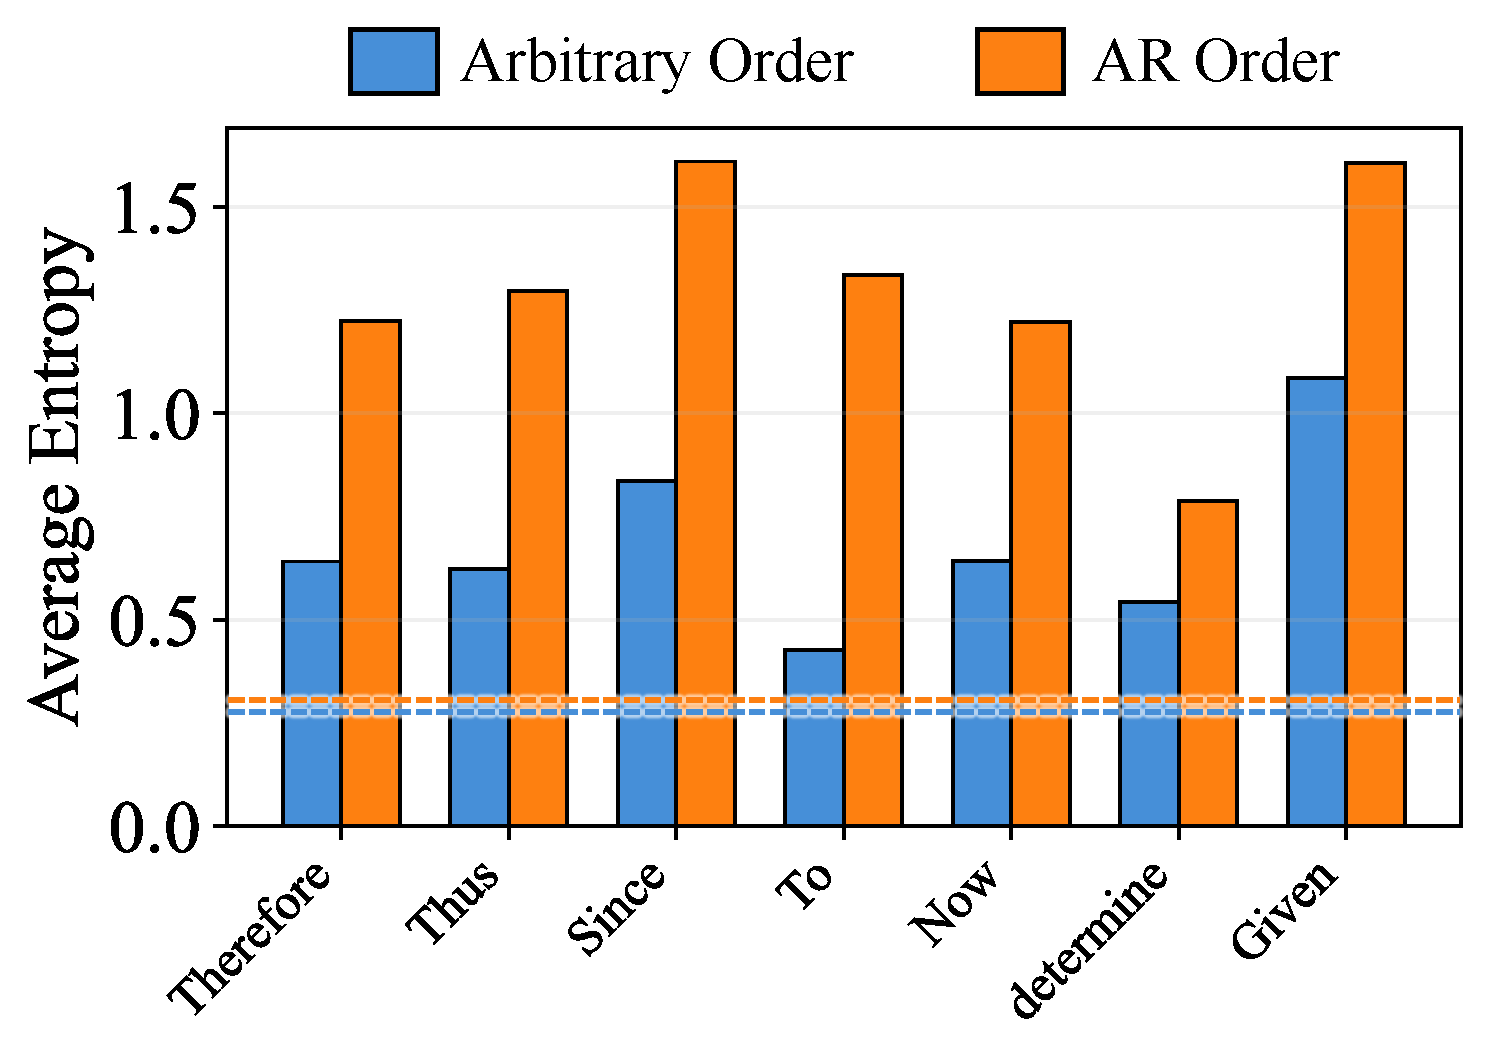
\includegraphics[width=\linewidth]{figures/entropy_bar_compare.pdf}
    \vskip -0.06in
    \caption{
        \textbf{Entropy degradation.} arbitrary order의 global average token entropy(점선)는 AR과 비슷한 수준을 유지하지만, logical forks(파란 막대)에서의 entropy는 크게 감소한다.
        결과는 LLaDA-Instruct로 MATH-500에서 측정했다.
        \label{fig:bypass_compare}
    }
    \vskip -0.14in
\end{wrapfigure}
\paragraph{``entropy degradation'' 현상.}
arbitrary order의 adaptive behavior는 이러한 logical forking tokens에 어떤 영향을 미치는가?
우리는 Figure~\ref{fig:bypass_compare}에서 이 tokens가 decoded될 때의 entropy를 측정한다(더 많은 결과는 Appendix~\ref{app:more_results_entropy_degradation}).
AR order에서는 이러한 tokens가 decoding될 때 일반적으로 높은 entropy를 유지하는데, 이는 여러 reasoning paths가 여전히 viable한 비교적 풍부한 branching point를 나타낸다~\cite{wang2025beyond}.
반대로 arbitrary order는 entropy의 급격한 감소를 보인다.
logical connectors를 뒤로 미룸으로써, model은 그들로 이어지는 logic connections를 결정하기 \emph{전에} 더 쉬운 future tokens 생성을 우선시한다.
model이 결국 bypass된 connectors를 채우기 위해 돌아오면, future context의 존재가 uncertainty를 크게 줄인다.
그 결과 model은 fork에서 open-ended navigational decision을 내리는 것이 아니라, 미리 정해진 conclusion으로 이어지는 gap을 bridge하기 위한 retrospective alignment에 가까운 일을 하게 된다.
우리는 이 현상을 \emph{entropy degradation}이라고 부른다.

\paragraph{Conclusion.}
요약하면, 우리의 발견은 일반 reasoning tasks에서 arbitrary order의 유연성이 inference-time exploitation을 exploration보다 의도치 않게 선호하게 만들 수 있음을 시사한다.
관찰된 entropy degradation은 이러한 경향의 정량적 지표 역할을 한다: uncertainty가 낮은 결정을 우선함으로써, model은 generation process의 초기에 자신의 trajectory를 특정 outcomes에 암묵적으로 anchor한다.
이는 solution space를 효과적으로 제약하여, single-shot coherence는 더 높일 수 있지만 complex problem-solving에 필요한 넓은 exploration을 제한할 수 있다.
표준 AR ordering은 causal chain을 엄격히 따름으로써 logical forks의 high-entropy 성질을 유지한다.
중요한 decision points를 우회할 수 없다는 점은 model이 다양한 reasoning branches에서 sample하도록 장려하며, 이는 reinforcement learning에 필수적인 solution coverage를 보존하는 데 도움이 된다.
